\documentclass{article}
\usepackage{booktabs} % for professional looking tables
\usepackage{array}
\usepackage[utf8]{inputenc}
\usepackage[russian]{babel}
\usepackage{siunitx}
\usepackage{csquotes}
\usepackage{url,amsmath,amssymb,fancybox,listings,pdfpages,caption,multicol,datetime,rotating, booktabs}
\usepackage{geometry}
\usepackage{graphicx}
\usepackage{subcaption}
\usepackage{multirow}
\usepackage{adjustbox}
\author{Николаев Владислав\\
	\texttt{v.nikolaev2@g.nsu.ru} \and
	Матяш Алексей\\
	\texttt{a.matyash@g.nsu.ru}}
\title{Определение константы диссоциации бромтимолового синего}
\begin{document}
	\maketitle
	\section{Изобестические точки}
	\begin{figure}[h]
		\centering
		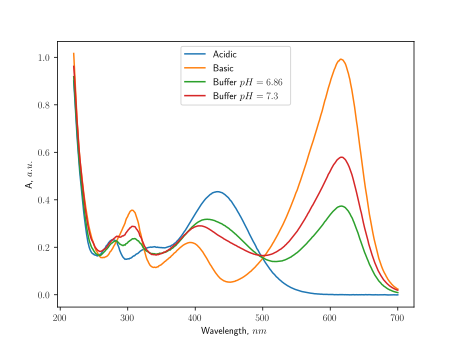
\includegraphics[width=1.0\textwidth]{4mg}
		\caption{Поглощение растворов при разных pH}
		\label{fig:isobest}
	\end{figure}
	Нашли изобестические точки как пересечения на \ref{fig:isobest}. Им соответствуют $\lambda_1=330\unit{\nano\meter}$ и $\lambda_2=500\unit{\nano\meter}$.
	
	Для них вычислили из всех известных концентраций коэффициенты молярной экстинкции (см. \ref{fig:eps330} \ref{fig:eps500})
	
	\begin{figure}[htbp]
		\centering
		\begin{subfigure}{0.49\textwidth}
			\centering
			\includegraphics[width=\textwidth]{eps330} 
			\caption{Расчёт $\epsilon_{330}$}
			\label{fig:eps330}
		\end{subfigure}
		\hfill
		\begin{subfigure}{0.49\textwidth}
			\centering
			\includegraphics[width=\textwidth]{eps500}  % Replace with your figure filename
			\caption{Расчёт $\epsilon_{500}$}
			\label{fig:eps500}
		\end{subfigure}
		\caption{Расчёт коэффициентов молярной экстинкции в изобестических точках}
		\label{fig:linearisobest}
	\end{figure}
	
	Получили:
	\begin{table}[htbp]
		\centering
		\caption{Коэффициенты молярной экстинкции в изобестических точках}  % Caption for the table
		\begin{tabular}{cc}  % Two columns with centered alignment
			\toprule
			\textbf{$\lambda$ (нм)} & \textbf{$\epsilon(\lambda)$} \\  % Table header
			\midrule
			330 & 8\,290 \\  % Data row
			500 & 6\,335 \\  % Data row
			\bottomrule
		\end{tabular}
	\end{table}
	
	\section{Расчёт $\,pK_a$}
	Затем "вытащили" оптические плотности растворов для рабочих длин волн, в качестве которых  взяли рекомендованные $615\unit{\nano\meter}$ и $\unit{433\nano\meter}$, так как судя по графику, на этой длине волны достаточная разница коэффициентов молярной экстинкции для аниона и дианиона.
	
	Вычислили коэффициенты молярной экстинкции, результаты занесли в таблицы \ref{tab:lam615} и \ref{tab:lam433}.
	\begin{table}[htbp]
		\centering
		\caption{Данные для индикатора при $\lambda = 615\unit{\nano\meter}$ }
		\resizebox{\textwidth}{!}{
			\begin{tabular}{>{\centering\arraybackslash}m{3cm} >{\centering\arraybackslash}m{3cm} >{\centering\arraybackslash}m{3cm} >{\centering\arraybackslash}m{3cm} >{\centering\arraybackslash}m{4cm}}
				\toprule
				\textbf{Форма индикатора} & \textbf{Номер раствора} & \textbf{C \unit{\mole/\liter}} & \textbf{$D_{615}$} & \textbf{Коэффициент экстинкции} \\
				\midrule
				\textbf{HA$^-$} & 1 & $5.13 \times 10^{-5}$ & $1.91 \times 10^{-3}$ & 27 \\
				& 2 & $3.84 \times 10^{-5}$ & $1.43 \times 10^{-3}$ & \\
				& 3 & $2.56 \times 10^{-5}$ & $2.13 \times 10^{-4}$ & \\
				& 4 & $1.28 \times 10^{-5}$ & $3.37 \times 10^{-4}$ & \\
				\textbf{A$^{2-}$} & 5 & $2.56 \times 10^{-5}$ & $9.92 \times 10^{-1}$ & 36 411 \\
				& 6 & $1.28 \times 10^{-5}$ & $4.76 \times 10^{-1}$ & \\
				& 7 & $6.41 \times 10^{-6}$ & $2.08 \times 10^{-1}$ & \\
				& 8 & $3.20 \times 10^{-6}$ & $1.20 \times 10^{-1}$ & \\
				\bottomrule
			\end{tabular}
		}
		\label{tab:lam615}
	\end{table}
	
	\vspace{1cm}
	
	\begin{table}[htbp]
		\centering
		\caption{Данные для индикатора при $\lambda = 433\unit{\nano\meter}$}
		\resizebox{\textwidth}{!}{
			\begin{tabular}{>{\centering\arraybackslash}m{3cm} >{\centering\arraybackslash}m{3cm} >{\centering\arraybackslash}m{3cm} >{\centering\arraybackslash}m{3cm} >{\centering\arraybackslash}m{4cm}}
				\toprule
				\textbf{Форма индикатора} & \textbf{Номер раствора} & \textbf{C (моль/л)} & \textbf{$D_{433}$} & \textbf{Коэффициент экстинкции} \\
				\midrule
				\textbf{HA$^-$} & 1 & $5.13 \times 10^{-5}$ & $9.07 \times 10^{-1}$ & 17 136 \\
				& 2 & $3.84 \times 10^{-5}$ & $6.66 \times 10^{-1}$ & \\
				& 3 & $2.56 \times 10^{-5}$ & $4.34 \times 10^{-1}$ & \\
				& 4 & $1.28 \times 10^{-5}$ & $2.12 \times 10^{-1}$ & \\
				\textbf{A$^{2-}$} & 5 & $2.56 \times 10^{-5}$ & $8.17 \times 10^{-2}$ & 2 987 \\
				& 6 & $1.28 \times 10^{-5}$ & $3.77 \times 10^{-2}$ & \\
				& 7 & $6.41 \times 10^{-6}$ & $1.42 \times 10^{-2}$ & \\
				& 8 & $3.20 \times 10^{-6}$ & $1.15 \times 10^{-2}$ & \\
				\bottomrule
			\end{tabular}
		}
		\label{tab:lam433}
	\end{table}
	
	Для растворов $3, 5, 9, 10$ вычислили значения логарифма коэффициента активности (см. таблицу \ref{tab:pka}).
	
	Притом так как ионную силу буферного раствора нельзя хоть сколько-то разумно оценить из одного только значения pH, воспользовались значениями ионной силы для некоторого буфера, который, в рамках работы, полагался стандартным (см. рис. \ref{fig:ionic_strength}).
	
	$$\lg{\frac{\gamma_{2-}}{\gamma_-}} = - \frac{0.509\cdot Z_{i-}^2\sqrt{I}}{1 + \sqrt{I}}$$
	
	$\,pK_a$ вычисляли по следующей формуле:
	$$\lg{K_a}=\lg{\frac{\alpha}{1-\alpha}}- pH + \lg{\frac{\gamma_{2-}}{\gamma_-}}$$
	
	Так как при длине волны $430\unit{\nano\meter}$ анион и дианион поглощают хотя и с заметно разной интенсивностью, но всё же разность коэффициентов молярной экстинкции не так велика (ср. таблицы \ref{tab:lam615} \ref{tab:lam433}), то расчёт $\alpha$ для этой длины волны провели, с учётом коэффициентов молярной экстинкции для обеих форм. Формула для расчёта:
	
	$$D=l\cdot C_0\cdot(\epsilon_{HA}+\alpha(\epsilon_{A}-\epsilon_{HA}))$$
	
	Видно, что $\alpha = \frac{D_A}{D_{HA}}$ является предельным случаем уравнения, представленного выше при $\epsilon_{HA} \rightarrow 0$, почему ей и воспользовались для расчёта доли дианиона для длины волны $615\unit{\nano\meter}$
	
	Стоит отметить, что вычисления константы ксилотности в условиях фактически полного протонирования или депротонирования формы нек корректно (точности измерений не хватает).
	\begin{figure}[h]
		\centering
		\includegraphics[width=0.8\textwidth]{ionic_strength}
		\caption{Ионная сила некоторого "стандартного" буфера}
		\label{fig:ionic_strength}
	\end{figure}
	
	
\begin{table}[htbp]
	\centering
	\caption{Параметры растворов при различных значениях pH}
	\begin{adjustbox}{width=\textwidth}
		\begin{tabular}{ccccccccccc}  % Ten columns for the data
			\toprule
			\multirow{2}{*}{\textbf{Номер раствора}} & \multirow{2}{*}{\textbf{pH}} & \multirow{2}{*}{\textbf{$I_c$ (M)}} & \multicolumn{2}{c}{\textbf{$D_{\lambda}$}} & \multicolumn{2}{c}{\textbf{$\alpha_{\lambda}$}} & \multicolumn{2}{c}{\textbf{$\lg{\frac{\alpha}{1-\alpha}}$}} & \multicolumn{2}{c}{\textbf{$pK_a$}} \\  
			\cmidrule(lr){4-5} \cmidrule(lr){6-7} \cmidrule(lr){8-9} \cmidrule(lr){10-11}
			&  &  & \textbf{433 \unit{\nano\meter}} & \textbf{615 \unit{\nano\meter}} & \textbf{433 \unit{\nano\meter}} & \textbf{615 \unit{\nano\meter}} & \textbf{433 \unit{\nano\meter}} & \textbf{615 \unit{\nano\meter}} & \textbf{433 \unit{\nano\meter}} & \textbf{615 \unit{\nano\meter}} \\  
			\midrule
			3  & 2.0  & $1.0 \times 10^{-2}$  & $4.34 \times 10^{-1}$ & $2.13 \times 10^{-4}$ & & &  \\ 
			5  & 12.0 & $1.0 \times 10^{-2}$  & $8.17 \times 10^{-2}$ & $9.92 \times 10^{-1}$ & & & & & &  \\ 
			9  & 6.8  & $1.8 \times 10^{-3}$  & $3.07 \times 10^{-1}$ & $3.73 \times 10^{-1}$ & $3.61 \times 10^{-1}$ & $3.76 \times 10^{-1}$ & $-2.48 \times 10^{-1}$ & $-2.19 \times 10^{-1}$ & 7.1 & 7.1 \\  
			10 & 7.3  & $1.2 \times 10^{-3}$  & $2.52 \times 10^{-1}$ & $5.78 \times 10^{-1}$ & $5.16 \times 10^{-1}$ & $5.83 \times 10^{-1}$ & $2.81 \times 10^{-2}$ & $1.46 \times 10^{-1}$ & 7.3 & 7.2 \\  
			\midrule
			\multicolumn{9}{r}{Среднее}  &  7.2 & 7.2 \\  % Average row
			\multicolumn{9}{r}{Справочные данные}  & \multicolumn{2}{c}{7.0}\\  % Reference data
			\bottomrule
		\end{tabular}
		\label{tab:pka}
	\end{adjustbox}
\end{table}
\textbf{Итог}: определили значение константы диссоциации индикатора бромтимолового синего по второй ступени при помощи спекрофотометрии. Результат по порядку величины совпал со справочными значениями. Предположительно, значительную погрешность вносит ионная сила раствора, которая не определялась экспериментально.

\pagebreak
\section{Литература}
\begin{itemize}
	\item Краткий справочник физико-химических величин (\textit{под ред. Равделя})
\end{itemize}
\end{document}
